%--------------------------------------------%
% Packages arranged by : Tsz Timmy Chan	     %
%                 Date : November 26th, 2016%
%--------------------------------------------%

\documentclass{TC}
\usepackage{TCcommon}

\title{TITLE HERE}	% Work Title Here.
\author{Tsz Timmy Chan}	% YOUR NAME HERE 

\usepackage[notes]{TCheader}
\usepackage{TCexamtitle}
%\renewcommand{\benediction}{" " - }
%\renewcommand{\quoteoftheday}{" " \\ - }
\begin{document}
Cones are intimately related to polytopes and polyhedra. In this narrative to discuss the main theorem of polytope theory, we will show how to embed both H-polyhedra and V-polyhedra of dimension $d$ into $\R^{d+1}$ as cones. This intimate relation between cones and polytopes is also the motivation later for the relationship between normal polytopes and rational cones.

 A cone in a vector space (or $\R^d$) is defined as the following:

\begin{definition}[Cone]
A set $C \subset \R^d$ is a cone if for every $ x \in C , \lambda x \in C \text{ for every } \lambda \geq 0$.
\end{definition}

Clearly, the intersection of cones is again a cone, and some trivial cases are the empty set $\{\emptyset\}$ and the whole space $\R^d$.

Given any set $K \subset \R^d$, we are also interested in the smallest cone that contains this set. Similar to the construction of the convex hull, the \emph{conical hull} can be characterized as the intersection of all the cones that contain $K$ or as non-negative linear combinations of all the elements of $K$:

\begin{definition}[Conical hull] Given a set $K \subseteq \R^d$, the conical hull of $K$, denoted $\mathrm{cone}(K)$, is the smallest cone that contains $K$, and 

\begin{align*}
\mathrm(K) &= \bigcap\{C \subseteq \R^d: K \subseteq C, C \text{ is a cone}\}, \\
			&= \{\lambda_1 x_1 + \cdots + \lambda_n x_n : \{ x_1,\ldots,x_k\} \subseteq K, \lambda_i \geq 0\}.
\end{align*}
In particular, we'll be interested in the case when $K$ is a finite set.
\end{definition}

\begin{figure}[h]
\centering
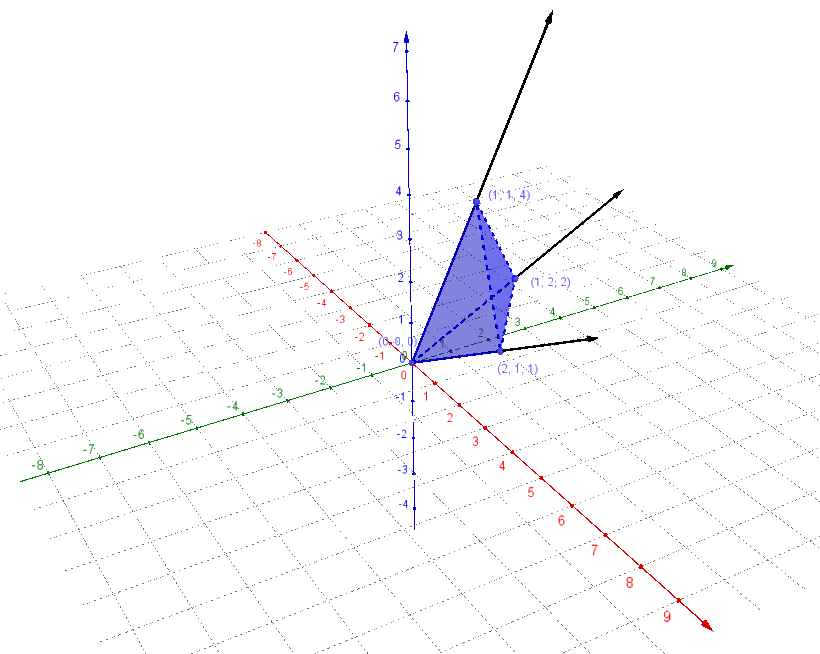
\includegraphics[width=.7\textwidth]{ExampleCone.png}
\caption{Example of $\mathrm{cone}(K)$ for some finite $K \subset \R^3$.}
\end{figure}

The \emph{Minkowski sum} of two sets $P, Q \subseteq \R^d$ is $P+Q = \{ p+q: p \in P, q\in Q\}$. With this operation, we can define a V-polyhedron as the Minkowski sum of the conical hull of a finite set of vectors and the convex hull of another finite set of vectors:

\begin{definition}[V-polyhedron] A \emph{V-polyhedron} denotes any finitely generated convex-conical combination, in other words, a set $P \subset \R^d$ of the form
$$P = \mathrm{conv}(V) + \mathrm{cone}(Y) $$
for some finite sets $V, Y \subset \R^d$.
\end{definition}

From this definition, a \emph{V-polytope} is a bounded \emph{V-polyhedron}. 

To draw the definitive relationship between the unique characterization of the V-polytope as the convex hull of finitely many points and H-polytope as the intersection of finite halfspaces, one strategy is to show that there exists a unique homogenous cone in dimension $d+1$, according to \cite{Ziegler}.

\subsection{Homogenization of Polyhedron} \label{homogenization_map}
The narrative in \cite{Ziegler} introduced the homogenization map, by simply adjoining an extra coordinate to the vectors with the intention to reduce the narrative to show that a V-polyhedra in $\R^d$ is also an H-polyhedra in $\R^d$ by associating a well-defined cone with each type in $\R^{d+1}$ in the following ways, with the goal of embedding the polyhedra in the plane $x_0 = 1$ and forming a cone to represent such a polyhedra without loss of information.

If $P_H$ is some $H$-polyhedron, i.e., $P_H = \{ x \in \R^d : Ax \leq z, A \in \R^{m\times d}, z \in \R^m\}$, we can create a cone in $\R^{d+1}$ by encoding the inequalities $a_i \mathbf x \leq z_i$ into $a_i\mathbf x \leq z_i x_0$ with $x_0 \geq 0$. More specifically, let  

\begin{equation} \label{H-homogenization_map}
C(P_H) =  \begin{bmatrix}
-1 & 0 & \cdots & 0 \\
-z_0 & a_{11} & \cdots & a_{1d} \\
\vdots & \vdots & \ddots & \vdots \\
-z_m & a_{m1} & \cdots & a_{md}
\end{bmatrix} \begin{bmatrix}
x_0 \\ x_1 \\ \vdots \\ x_d
\end{bmatrix} \leq \begin{bmatrix}
0 \\ 0 \\ \vdots \\0
\end{bmatrix}.
\end{equation}
Note that when $x_0 = 1$, we have the polytope $P$ in the plane intersecting $C(P)$, and that $C(P)$ and $P$ are both H-polyhedra.

Similarly, if $P_V$ is some V-polyhedra where $P_V = \mathrm{conv}(U) + \mathrm{cone}(W)$ for some finite sets $U,W \subset \R^d$, we can form a $C(P_V)$ in $\R^{d+1}$ as follows: 

\begin{equation}\label{V-homogenization_map}
C(P_V) = \mathrm{cone}\left(\begin{bmatrix}
1 \\ u_{11} \\ \vdots \\ u_{d1}
\end{bmatrix}, \cdots , 
\begin{bmatrix}
1 \\ u_{1j} \\ \vdots \\ u_{dj}
\end{bmatrix} , \begin{bmatrix}
0 \\ w_{11} \\ \vdots \\ w_{d1}
\end{bmatrix}, \cdots , 
\begin{bmatrix}
0 \\ w_{1k} \\ \vdots \\ w_{dk}
\end{bmatrix}\right),
\end{equation}

The construction creates a cone in $\R^{d+1}$, as the conical hull of these vectors, with the property that $$ P = \left \{ \mathbf x \in \R^d : \begin{bmatrix}
1 \\ \mathbf x
\end{bmatrix} \in C(P)\right \}.$$

And the points at infinity (the part of $P$ that is defined using the conical hull of $Y$) is recorded on the plane $x_0 = 0$.

\begin{theorem}[Main theorem of polytope theory: Cone Version] \label{Cone_Theorem}


A cone $C \subseteq \R^d$ is finitely generated combination of vectors $$ C = \mathrm{cone}(V) \text{ for some finite } V \subset \R^d $$
if and only if it is a finite intersection of closed linear halfspaces
$$ C = \{x \in \R^d : Ax \leq 0\} \text{ for some } A \in \R^{m \times d}\} .$$
\end{theorem}

The proof of this theorem is nontrivial and can be found in Section 1.3 of \cite{Ziegler}. With the information from Theorem \ref{Cone_Theorem}, and the aforementioned construction of cones using V-polyhedra and H-polyhedra, together they imply (through the construction of the homogenization map) the following theorem. 


\begin{theorem}[Main Theorem of Polytope Theory: Polyhedral version]
A subset $P \subseteq \R^d$ is the Minskowski sum of the convex hull of a finite point set and the conical hull of another finite point set (a \emph{V-polyhedron}) $$ P = \mathrm{conv}(V) + \mathrm{cone}(Y) \text{, for some finite } V,Y \subset \R^d$$ if and only if it is a finite intersection of halfspaces (an \emph{H-polytope})
$$ P = \{x \in \R^d : A x  = z \text{, for some } A \in \R^{m\times d}, z \in \R^m \}.$$

\end{theorem}

And the above, once we set the "bounded" condition, is the Polytope version.

\subsection{Recession Cones for Convex Sets}
Given a convex set $A \subset V$ where $V$ is an inner product space (in our case, $V = \R^d$). A vector $y$ is a \emph{direction of recession} if starting at any $x$ in $A$ and going indefinitely along $y$, we never cross the relative boundary of $A$ to points outside $A$. Formally speaking:


\begin{definition}[Recession Cone of a Convex Set]
Given $A \subset V$ is convex, then the \emph{recession cone} of $A$ is defined as:
$$ \mathrm{rec}(A) = \{y \in V: x + \lambda y \in A \text{ for every } x \in A, \lambda \geq 0\}.$$
\end{definition}


Note that $\vec 0$ is always in $\mathrm{rec}(A)$, and that for a bounded set $A$, the recession cone $\mathrm{rec}(A)$ is just the zero vector. 

Similarly, a vector $y$ is in the \emph{linearity space} of the convex set $A \subset V$ if starting at any $x \in A$ and going indefinitely along $y$ in BOTH directions, we can never cross the relative boundary of $A$ to points outside of $A$. Formally:

\begin{definition}[Linearity Space of a Convex Set] 
Given $A \subset V$ is convex, then  the \emph{linearity space} of $A$ is defined as $$\mathrm{lineal}(A) = \{y \in V: x + \lambda y \in A \text{ for every } x \in A, \lambda \in \R\}.$$
\end{definition}

Note that the linearity space is a vector subspace of $\R^d$ in its own right, and the set $A$ is a strict subset of $\R^d$ if and only if $\dim(\mathrm{lineal}(A)) < d$. If we construct a vector subspace $W$ such that  $\{\vec 0\} = W \cap \mathrm{lineal}(A)$ and $W + \mathrm{lineal}(A) = \R^d$ by choosing basis elements that are linearly independent from all basis elements of $\mathrm{lineal}(A)$ (from linear algebra, $\dim W = d - \dim(\mathrm{lineal}(A))$) and then using this complement vector subspace $W$, we can decompose a convex set with non-empty linearity space into two parts by a Minkowski sum:
$$ P = \mathrm{lineal}(P) + (P \cap W)$$
where the linearity space of $(P \cap W)$ is zero. In other words, $(P \cap W)$ is a convex set that does not contain any lines. 

\begin{definition}[Pointed polyhedra]
A polyhedra $P$ is pointed if $\mathrm{lineal}(P)=\{0\}$; in other words, a polyhedra is pointed if it does not contain any lines. 
\end{definition}

Another perspective: a polyhedra $P$ is pointed whenever there exists some affine halfspace that strictly contains $P$.


\end{document}